%
% A header that lets you compile a chapter by itself, or inside a larger document.
% Adapted from http://stackoverflow.com/questions/3655454/conditional-import-in-latex
%
%
%Use \inbpdocument and \outbpdocument in your individual files, in place of \begin{document} and \end{document}. In your main file, put in a \def \ismaindoc {} before including or importing anything.
%
% David Duvenaud
% June 2011
% 
% ======================================
%
%


\ifx\ismaindoc\undefined
	\newcommand{\inbpdocument}{
		\def \ismaindoc {}
		% Use this header if we are compiling by ourselves.
		\documentclass[a4paper,11pt,authoryear,index]{common/PhDThesisPSnPDF}
		
%\usepackage{draftwatermark}
%\SetWatermarkLightness{0.95}

% ******************************************************************************
% ****************************** Custom Margin *********************************

% Add `custommargin' in the document class options to use this section
% Set {innerside margin / outerside margin / topmargin / bottom margin}  and
% other page dimensions

\ifsetMargin
\else
    \RequirePackage[left=37mm,right=30mm,top=35mm,bottom=30mm]{geometry}
    \setFancyHdr % To apply fancy header after geometry package is loaded
\fi


%\chead{Unfinished draft}
%\cfoot{\texttt{Unfinished draft - compiled on \today{} at \currenttime}}

% *****************************************************************************
% ******************* Fonts (like different typewriter fonts etc.)*************

% Add `customfont' in the document class option to use this section

\ifsetFont
\else
    % Set your custom font here and use `customfont' in options. Leave empty to
    % load computer modern font (default LaTeX font).  

    \RequirePackage{libertine} 
\fi

% *****************************************************************************
% *************************** Bibliography  and References ********************

%\usepackage{cleveref} %Referencing without need to explicitly state fig /table

% Add `custombib' in the document class option to use this section
\ifsetBib % True, Bibliography option is chosen in class options
\else % If custom bibliography style chosen then load bibstyle here

   \RequirePackage[square, sort, numbers, authoryear]{natbib} % CustomBib

% If you would like to use biblatex for your reference management, as opposed to the default `natbibpackage` pass the option `custombib` in the document class. Comment out the previous line to make sure you don't load the natbib package. Uncomment the following lines and specify the location of references.bib file

% \RequirePackage[backend=biber, style=numeric-comp, citestyle=numeric, sorting=nty, natbib=true]{biblatex}
% \bibliography{References/references} %Location of references.bib only for biblatex

\fi


% changes the default name `Bibliography` -> `References'
\renewcommand{\bibname}{References}


% *****************************************************************************
% *************** Changing the Visual Style of Chapter Headings ***************
% Uncomment the section below. Requires titlesec package.

%\RequirePackage{titlesec}
%\newcommand{\PreContentTitleFormat}{\titleformat{\chapter}[display]{\scshape\Large}
%{\Large\filleft{\chaptertitlename} \Huge\thechapter}
%{1ex}{}
%[\vspace{1ex}\titlerule]}
%\newcommand{\ContentTitleFormat}{\titleformat{\chapter}[display]{\scshape\huge}
%{\Large\filleft{\chaptertitlename} \Huge\thechapter}{1ex}
%{\titlerule\vspace{1ex}\filright}
%[\vspace{1ex}\titlerule]}
%\newcommand{\PostContentTitleFormat}{\PreContentTitleFormat}
%\PreContentTitleFormat


% *****************************************************************************
% **************************** Custom Packages ********************************
% *****************************************************************************


% ************************* Algorithms and Pseudocode **************************

%\usepackage{algpseudocode} 


% ********************Captions and Hyperreferencing / URL **********************

% Captions: This makes captions of figures use a boldfaced small font. 
%\RequirePackage[small,bf]{caption}

\RequirePackage[labelsep=space,tableposition=top]{caption} 
%\renewcommand{\figurename}{Figure} %to support older versions of captions.sty
\captionsetup{belowskip=12pt,aboveskip=4pt}

% ************************ Formatting / Footnote *******************************

%\usepackage[perpage]{footmisc} %Range of footnote options 


% ****************************** Line Numbers **********************************

%\RequirePackage{lineno}
%\linenumbers

% ************************** Graphics and figures *****************************

%\usepackage{rotating}
%\usepackage{wrapfig}
%\usepackage{float}
\usepackage{subfig} %note: subfig must be included after the `caption` package. 


% ********************************* Table **************************************

%\usepackage{longtable}
%\usepackage{multicol}
%\usepackage{multirow}
%\usepackage{tabularx}


% ***************************** Math and SI Units ******************************

\usepackage{amsfonts}
\usepackage{amsmath}
\usepackage{amssymb}
%\usepackage{siunitx} % use this package module for SI units


% ******************************************************************************
% ************************* User Defined Commands ******************************
% ******************************************************************************

% *********** To change the name of Table of Contents / LOF and LOT ************

%\renewcommand{\contentsname}{My Table of Contents}
%\renewcommand{\listfigurename}{List of figures}
%\renewcommand{\listtablename}{List of tables}


% ********************** TOC depth and numbering depth *************************

\setcounter{secnumdepth}{2}
\setcounter{tocdepth}{2}

% ******************************* Nomenclature *********************************

% To change the name of the Nomenclature section, uncomment the following line

%\renewcommand{\nomname}{Symbols}


% ********************************* Appendix ***********************************

% The default value of both \appendixtocname and \appendixpagename is `Appendices'. These names can all be changed via: 

%\renewcommand{\appendixtocname}{List of appendices}
%\renewcommand{\appendixname}{Appndx}

		% All my custom preamble stuff.  Shouldn't overlap with anything in official-preamble


% Paths to figure and table directories.
\newcommand{\symmetryfigsdir}{figures/symmetries}
\newcommand{\topologyfiguresdir}{figures/topology}
\newcommand{\infinitefiguresdir}{figures/infinite}
\newcommand{\grammarfiguresdir}{figures/grammar}
\newcommand{\introfigsdir}{figures/intro}
\newcommand{\gplvmfiguresdir}{figures/gplvm}
\newcommand{\warpedfiguresdir}{figures/warped-mixtures}
\newcommand{\deeplimitsfiguresdir}{figures/deep-limits}
\newcommand{\quadraturefigsdir}{figures/quadrature}
\newcommand{\additivefigsdir}{figures/additive}
\newcommand{\decompfigsdir}{figures/decomp}
\newcommand{\examplefigsdir}{figures/worked-example}


\usepackage{bm}  % for warped mixtures - is this necessary?
\usepackage{booktabs}
\usepackage{tabularx}
\usepackage{multirow}
\usepackage{datetime}
\renewcommand{\tabularxcolumn}[1]{>{\arraybackslash}m{#1}}
\usepackage{relsize}
\usepackage{graphicx}
\usepackage{amsmath,amssymb,textcomp}
\usepackage{nicefrac}
\usepackage{amsthm}
\usepackage{tikz}
\usetikzlibrary{arrows}
\usetikzlibrary{calc}
\usepackage{nth}
\usepackage{rotating}
\usepackage{array}
\usepackage{fp}
\usepackage[hyperpageref]{backref}
\def\foo{\hspace{\fill}\mbox{}\linebreak[0]\hspace*{\fill}}
\renewcommand*{\backref}[1]{}
\renewcommand*{\backrefalt}[4]{%
\ifcase #1 %
%
\or
\foo(page #2)%
\else
\foo(pages #2)%
\fi
}

\usepackage{cleveref}
\crefname{equation}{equation}{equations}


%% For submission, make all render blank.
%%%%%%%%%%%%%%%%%%%%%%%%%%%%%%%%%%%%%%%%%%%%%%%%%%%%%%%%%%
%%%% EDITING HELPER FUNCTIONS  %%%%%%%%%%%%%%%%%%%%%%%%%%%
%%%%%%%%%%%%%%%%%%%%%%%%%%%%%%%%%%%%%%%%%%%%%%%%%%%%%%%%%%

%% NA: needs attention (rough writing whose correctness needs to be verified)
%% TBD: instructions for how to fix a gap ("Describe the propagation by ...")
%% PROBLEM: bug or missing crucial bit 

%% use \fXXX versions of these macros to put additional explanation into a footnote.  
%% The idea is that we don't want to interrupt the flow of the paper or make it 
%% impossible to read because there are a bunch of comments.

%% NA's (and TBDs, those less crucially) should be written so 
%% that they flow with the text.

\definecolor{WowColor}{rgb}{.75,0,.75}
\definecolor{SubtleColor}{rgb}{0,0,.50}

% inline
\newcommand{\NA}[1]{\textcolor{SubtleColor}{ {\tiny \bf ($\star$)} #1}}
\newcommand{\LATER}[1]{\textcolor{SubtleColor}{ {\tiny \bf ($\dagger$)} #1}}
\newcommand{\TBD}[1]{\textcolor{SubtleColor}{ {\tiny \bf (!)} #1}}
\newcommand{\PROBLEM}[1]{\textcolor{WowColor}{ {\bf (!!)} {\bf #1}}}

% as margin notes

\newcounter{margincounter}
\newcommand{\displaycounter}{{\arabic{margincounter}}}
\newcommand{\incdisplaycounter}{{\stepcounter{margincounter}\arabic{margincounter}}}

\newcommand{\fTBD}[1]{\textcolor{SubtleColor}{$\,^{(\incdisplaycounter)}$}\marginpar{\tiny\textcolor{SubtleColor}{ {\tiny $(\displaycounter)$} #1}}}

\newcommand{\fPROBLEM}[1]{\textcolor{WowColor}{$\,^{((\incdisplaycounter))}$}\marginpar{\tiny\textcolor{WowColor}{ {\bf $\mathbf{((\displaycounter))}$} {\bf #1}}}}

\newcommand{\fLATER}[1]{\textcolor{SubtleColor}{$\,^{(\incdisplaycounter\dagger)}$}\marginpar{\tiny\textcolor{SubtleColor}{ {\tiny $(\displaycounter\dagger)$} #1}}}

%\renewcommand{\LATER}[1]{}
%\renewcommand{\fLATER}[1]{}
%\renewcommand{\TBD}[1]{}
%\renewcommand{\fTBD}[1]{}
%\renewcommand{\PROBLEM}[1]{}
%\renewcommand{\fPROBLEM}[1]{}
%\renewcommand{\NA}[1]{}


% HUMBLE WORDS: shown slightly smaller when in normal text
% Thanks to Christian Steinruecken!

% HUMBLE WORDS: shown slightly smaller when in normal text
%
\makeatletter%
%\def\@humbleformat#1{{\fontsize{}{1em}\selectfont #1}}
%\def\@humbleformat#1{\textsmaller{#1}}%
\newlength{\nonHumbleHeight}
\def\@humbleformat#1{{\settoheight{\nonHumbleHeight}{#1}\resizebox{!}{0.94\nonHumbleHeight}{#1}}}%
\def\@idxhumbleformat#1{{\relscale{0.95}{#1}}}%
%\def\@humbleformat#1{{#1}}%
\def\declareHumble#1#2{%
  \expandafter\def\csname #1\endcsname{\@humbleformat{#2}}%
  \expandafter\def\csname s#1\endcsname{{#2}}%
  \expandafter\def\csname idx#1\endcsname{{\@idxhumbleformat{#2}}}%
}%
\def\humble#1{\@humbleformat{#1}}%
\def\idxhumble#1{\@idxhumbleformat{#1}}%
\makeatother%

% Convenient indexing for humble abbreviations
\def\humbleindex#1#2{\index{#1@\idxhumble{#1}}}



% TODO: Clean up duplicates
\declareHumble{ANOVA}{ANOVA}
\declareHumble{ARD}{ARD}
\declareHumble{BIC}{BIC}
\declareHumble{BMC}{BMC}
\declareHumble{bq}{BQ}
\declareHumble{CRP}{CRP}
\declareHumble{dirpro}{DP}
\declareHumble{HDMR}{HDMR}
\declareHumble{GAM}{GAM}
\declareHumble{GEM}{GEM}
\declareHumble{GMM}{GMM}
\declareHumble{gplvm}{GP-LVM}
\declareHumble{gpml}{GPML}
\declareHumble{GPML}{GPML}
\declareHumble{gprn}{GPRN}
\declareHumble{gpt}{GP}
\declareHumble{gp}{GP}
\declareHumble{HKL}{HKL}
\declareHumble{HMC}{HMC}
\declareHumble{ibp}{IBP}
\declareHumble{iGMM}{iGMM}
\declareHumble{iwmm}{iWMM}
\declareHumble{kCP}{CP}
\declareHumble{kCW}{CW}
\declareHumble{kC}{C}
\declareHumble{KDE}{KDE}
\declareHumble{kLin}{Lin}
\declareHumble{KPCA}{KPCA}
\declareHumble{kPer}{Per}
\declareHumble{kRQ}{RQ}
\declareHumble{kSE}{SE}
\declareHumble{kWN}{WN}
\declareHumble{Lin}{Lin}
\declareHumble{LBFGS}{L-BFGS}
\declareHumble{mcmc}{MCMC}
\declareHumble{MKL}{MKL}
\declareHumble{MLP}{MLP}
\declareHumble{MSE}{MSE}
\declareHumble{Per}{Per}
\declareHumble{RMSE}{RMSE}
\declareHumble{RQ}{RQ}
\declareHumble{SBQ}{SBQ}
\declareHumble{seard}{SE-ARD}
\declareHumble{sefull}{SE-\textnormal{full}}
\declareHumble{SEGP}{SE-GP}
\declareHumble{SE}{SE}
\declareHumble{SNR}{SNR}
\declareHumble{SSANOVA}{SS-ANOVA}
\declareHumble{SVM}{SVM}

\newcommand{\kSig}{\boldsymbol\sigma}

\def\subexpr{{\cal S}}
\def\baseker{{\cal B}}
\def\numWinners{k}

\def\ie{i.e.\ }
\def\eg{e.g.\ }
\def\etc{etc.\ }
\let\oldemptyset\emptyset
\let\emptyset 0




% Unify notation between neural-net land and GP-land.
\newcommand{\hphi}{h}
\newcommand{\hPhi}{\vh}
\newcommand{\walpha}{w}
\newcommand{\wboldalpha}{\bw}
\newcommand{\wcapalpha}{\vW}
\newcommand{\lengthscale}{w}

\newcommand{\layerindex}{\ell}



\newcommand{\gpdrawbox}[1]{
\setlength\fboxsep{0pt}
\hspace{-0.15in} 
\fbox{
\includegraphics[width=0.464\columnwidth]{\deeplimitsfiguresdir/deep_draws/deep_gp_sample_layer_#1}
}}



\newcommand{\procedurename}{ABCD}
\newcommand{\genText}[1]{{\sf #1}}



\newcommand{\asdf}{$^{\textnormal{th}}$}

\newcommand{\binarysum}{\sum_{\bf{x} \in \{0,1\}^D}}
\newcommand{\expect}{\mathbb{E}}
\newcommand{\expectargs}[2]{\mathbb{E}_{#1} \left[ {#2} \right]}
\newcommand{\var}{\mathbb{V}}
\newcommand{\varianceargs}[2]{\mathbb{V}_{#1} \left[ {#2} \right]}
\newcommand{\cov}{\operatorname{cov}}
\newcommand{\Cov}{\operatorname{Cov}}
\newcommand{\covargs}[2]{\cov \left[ {#1}, {#2} \right]}
\newcommand{\variance}{\mathbb{V}}
\newcommand{\vecop}[1]{\operatorname{vec} \left( {#1} \right)}

\newcommand{\covarianceargs}[2]{\Cov_{#1} \left[ {#2} \right]}
\newcommand{\colvec}[2]{\left[ \begin{array}{c} {#1} \\ {#2} \end{array} \right]}
\newcommand{\tbtmat}[4]{\left[ \begin{array}{cc} {#1} & {#2} \\ {#3} & {#4} \end{array} \right]}

%\newcommand{\covskinny}[2]{\var\!\left(#1\middle\vert#2\right)} 

\newcommand{\acro}[1]{{\humble{#1}}}
%\newcommand{\vect}[1]{\boldsymbol{#1}}
\newcommand{\vect}[1]{{\bf{#1}}}
\newcommand{\mat}[1]{\mathbf{#1}}
\newcommand{\pderiv}[2]{\frac{\partial #1}{\partial #2}}
\newcommand{\npderiv}[2]{\nicefrac{\partial #1}{\partial #2}}

\newcommand{\pha}{^{\phantom{:}}}

\newcommand{\argmin}{\operatornamewithlimits{argmin}}
\newcommand{\argmax}{\operatornamewithlimits{argmax}}

% The following designed for probabilities with long arguments

\newcommand{\Prob}[2]{P\!\left(\,#1\;\middle\vert\;#2\,\right)}
\newcommand{\ProbF}[3]{P\!\left(\,#1\!=\!#2\;\middle\vert\;#3\,\right)}
\newcommand{\p}[2]{p\!\left(#1\middle\vert#2\right)}
\newcommand{\po}[1]{p\!\left(#1\right)}
\newcommand{\pF}[3]{p\!\left(\,#1\!=\!#2\;\middle\vert\;#3\,\right)} 
\newcommand{\mean}[2]{{m}\!\left(#1\middle\vert#2\right)}



\newcommand{\valpha}{\boldsymbol{\alpha}}
\newcommand{\va}{\vect{a}}
\newcommand{\vA}{\vect{A}}
\newcommand{\vB}{\mat{B}}
\newcommand{\vb}{\vect{b}}
\newcommand{\vC}{\mat{C}}
\newcommand{\vc}{\vect{c}}
\newcommand{\vecf}{\boldsymbol{f}}
\newcommand{\vell}{\vect{\ell}}
\newcommand{\vepsilon}{\boldsymbol{\epsilon}}
\newcommand{\veps}{\boldsymbol{\epsilon}}
\newcommand{\ve}{\boldsymbol{\epsilon}}
\newcommand{\vf}{\vecf}
\newcommand{\vg}{\vect{g}}
\newcommand{\vh}{\vect{h}}
\newcommand{\vI}{\mat{I}}
\newcommand{\vK}{\mat{K}}
\newcommand{\vk}{\vect{k}}
\newcommand{\vL}{\mat{L}}
\newcommand{\vl}{\vect{l}}
\newcommand{\vmu}{\boldsymbol{\mu}}
\newcommand{\vone}{\vect{1}}
\newcommand{\vphi}{\boldsymbol{\phi}}
\newcommand{\vpi}{\boldsymbol{\pi}}
\newcommand{\vq}{\vect{q}}
\newcommand{\vR}{\mat{R}}
\newcommand{\vr}{\vect{r}}
\newcommand{\vsigma}{\boldsymbol{\sigma}}
\newcommand{\vSigma}{\mat{\Sigma}}
\newcommand{\vS}{\mat{S}}
\newcommand{\vs}{\vect{s}}
\newcommand{\vtheta}{\boldsymbol{\theta}}
\newcommand{\vu}{\vect{u}}
\newcommand{\vV}{\mat{V}}
\newcommand{\vW}{\mat{W}}
\newcommand{\vw}{\vect{w}}
\newcommand{\vX}{\mat{X}}
\newcommand{\vx}{\vect{x}}
\newcommand{\vY}{\mat{Y}}
\newcommand{\vy}{\vect{y}}
\newcommand{\vzero}{\vect{0}}
\newcommand{\vZ}{\mat{Z}}
\newcommand{\vz}{\vect{z}}


\newcommand{\netweights}{\alpha}
\newcommand{\vnetweights}{\valpha}

\newcommand{\He}{\mathcal{H}}
\newcommand{\normx}[2]{\left\|#1\right\|_{#2}}
\newcommand{\Hnorm}[1]{\normx{#1}{\He}}
\newcommand{\mmd}{{\rm MMD}}


\newcommand{\mf}{\bar{\vf}}

%\newcommand{\mf}{\mu} %{\bar{\ell}}
\newcommand{\lf}{f} % Likelihood function
\newcommand{\st}{_\star}

% from simpler log-bq writeup
\newcommand{\lftwo}{{\log \ell}}
\newcommand{\mftwo}{{\bar \ell}}
\newcommand{\loggp}{{\log\acro{GP}}}%| \bX, \vy )}}
\newcommand{\loggpdist}{{\acro{GP}(\lftwo)}}%| \vX, \vy )}}


\newcommand{\inv}{^{{\mathsmaller{-1}}}}
\newcommand{\tohalf}{^{{\mathsmaller{\nicefrac{1}{2}}}}}

\newcommand{\Normal}{\mathcal{N}}
\newcommand{\N}[3]{\mathcal{N}\!\left(#1 \middle| #2,#3\right)}
\newcommand{\Nt}[2]{\mathcal{N}\!\left(#1,#2\right)}
\newcommand{\NT}[2]{\mathcal{N}\!\left(#1,#2\right)}
\newcommand{\GPdist}[3]{\mathcal{GP}\!\left(#1 \, \middle| \, #2, #3 \right)}
\newcommand{\bN}[3]{\mathcal{N}\big(#1 \middle| #2,#3\big)}
\newcommand{\boldN}[3]{\text{\textbf{\mathcal{N}}}\big(#1;#2,#3\big)}
\newcommand{\ones}[1]{\mat{1}_{#1}}
\newcommand{\eye}[1]{\mat{E}_{#1}}
\newcommand{\tra}{^{\mathsf{T}}}
%\newcommand{\tra}{^{\top}}
%\mathsf{T}
\newcommand{\trace}{\operatorname{tr}}
\newcommand{\shift}{\operatorname{shift}}
\renewcommand{\mod}{\operatorname{mod}}
\newcommand{\deq}{:=}
\newcommand{\oneofk}{\operatorname{one-of-k}}
%\newcommand{\degree}{^\circ}

\newcommand{\GPt}[2]{\mathcal{GP}\!\left(#1,#2\right)}
%\newcommand{\GPt}[2]{\gp\!\left(#1,#2\right)}

\DeclareMathOperator{\tr}{tr}
\DeclareMathOperator{\chol}{chol}
\DeclareMathOperator{\diag}{diag}

\newenvironment{narrow}[2]{%
  \begin{list}{}{%
  \setlength{\topsep}{0pt}%
  \setlength{\leftmargin}{#1}%
  \setlength{\rightmargin}{#2}%
  \setlength{\listparindent}{\parindent}%
  \setlength{\itemindent}{\parindent}%
  \setlength{\parsep}{\parskip}}%
\item[]}{\end{list}}



\newcommand{\dist}{\ \sim\ }
\def\given{\,|\,}

% Table stuff
\newcolumntype{C}[1]{>{\centering\let\newline\\\arraybackslash\hspace{0pt}}m{#1}}
\newcolumntype{L}[1]{>{\raggedright\let\newline\\\arraybackslash\hspace{0pt}}m{#1}}
\newcolumntype{R}[1]{>{\raggedleft\let\newline\\\arraybackslash\hspace{0pt}}m{#1}}


\def\ie{i.e.\ }
\def\eg{e.g.\ }
\def\iid{i.i.d.\ }
%\def\simiid{\sim_{\mbox{\tiny iid}}}
\def\simiid{\overset{\mbox{\tiny iid}}{\sim}}
\def\simind{\overset{\mbox{\tiny \textnormal{ind}}}{\sim}}
\def\eqdist{\stackrel{\mbox{\tiny d}}{=}}
%\newcommand{\distas}[1]{\mathbin{\overset{#1}{\kern \z@ \sim}}}
%TODO: fix this - it worked outside the thesis!
\newcommand{\distas}[1]{\mathbin{\overset{#1}{\sim}}}

\def\Reals{\mathbb{R}}

\def\Uniform{\mbox{\rm Uniform}}
\def\Bernoulli{\mbox{\rm Bernoulli}}
\def\GP{\mathcal{GP}}
\def\GPLVM{\mathcal{GP-LVM}}




% Kernel stuff

\def\iva{\vect{\inputVar}}
\def\ivaone{\inputVar}
\def\inputVar{x}
\def\InputVar{X}
\def\InputSpace{\mathcal{X}}
\def\outputVar{y}
\def\OutputSpace{\mathcal{Y}}
\def\function{f}
\def\kernel{k}
\def\KernelMatrix{K}
\def\SumKernel{\sum}
\def\ProductKernel{\prod}
\def\expression{e}
\def\feat{\vh}

\newcommand{\kerntimes}{ \! \times \!}
\newcommand{\kernplus}{ \, + \,}


% Proof stuff
\theoremstyle{plain}
\newtheorem{theorem}{Theorem}[section]
\newtheorem{lemma}[theorem]{Lemma}
\newtheorem{prop}[theorem]{Proposition}
\newtheorem{proposition}{Proposition}
\newtheorem*{cor}{Corollary}

% For infinite bq
\newcommand{\iv}{\theta}
\newcommand{\viv}{\vtheta}

% For intro chapter
\newcommand{\funcval}{\vf(\vX)}
\newcommand{\testpoint}{{\vx^\star}}

\newcommand{\underwrite}[2]{{\underbrace{#1}_{\textnormal{#2}}}}



% For kernel figures
\newcommand{\fhbig}{2cm}%
\newcommand{\fwbig}{3cm}%
\newcommand{\kernpic}[1]{\includegraphics[height=\fhbig,width=\fwbig]{\grammarfiguresdir/structure_examples/#1}}%
\newcommand{\kernpicr}[1]{\rotatebox{90}{\includegraphics[height=\fwbig,width=\fhbig]{\grammarfiguresdir/structure_examples/#1}}}%
\newcommand{\addkernpic}[1]{{\includegraphics[height=\fhbig,width=\fwbig]{\grammarfiguresdir/additive_multi_d/#1}}}%
\newcommand{\largeplus}{\tabbox{{\Large+}}}%
\newcommand{\largeeq}{\tabbox{{\Large=}}}%
\newcommand{\largetimes}{\tabbox{{\Large$\times$}}}%
\newcommand{\fixedx}{$x$ (with $x' = 1$)}%


		% ************************ Thesis Information & Meta-data **********************

%% The title of the thesis
%\title{Structured Gaussian Process Models} 
%\title{Automatic Model Construction \\ through \\ Structured Gaussian Processes}
%\title{Automatic Model-Building \\ through \\ Structured Gaussian Processes}
%\title{Automatic Modeling \\ with \\ Structured Gaussian Processes}    
\title{Automatic Model Construction \\ with Gaussian Processes}
%\title{Automatic Model Construction}
%\title{Automating Statistical Model Construction}


%\texorpdfstring is used for PDF metadata. Usage:
%\texorpdfstring{LaTeX_Version}{PDF Version (non-latex)} eg.,
%\texorpdfstring{$sigma$}{sigma}

%% The full name of the author
\author{David Kristjanson Duvenaud}

%% Department (eg. Department of Engineering, Maths, Physics)
%\dept{Department of Engineering}

%% University and Crest
\university{University of Cambridge}
\crest{
\includegraphics[width=0.25\textwidth]{University_Crest}}

%% You can redefine the submission text:
% Default as per the University guidelines: This dissertation is submitted for
% the degree of Doctor of Philosophy
%\renewcommand{\submissiontext}{change the default text here if needed}

%% Full title of the Degree 
\degree{Doctor of Philosophy}
 
%% College affiliation (optional)
\college{Pembroke College}

%% Submission date
\degreedate{June 2014} 

%% Meta information
\subject{LaTeX} \keywords{{LaTeX} {PhD Thesis} {Engineering} {University of Cambridge}}



		\begin{document}
	}	
	\newcommand{\outbpdocument}[1]{

		% Fake chapters so references aren't broken
\label{ch:intro}                
\label{ch:kernels}
\label{ch:grammar}
\label{ch:description}
\label{ch:additive}
\label{ch:deeplimits}
\label{ch:discussion}
		%\bibliographystyle{common/CUEDthesis}
		\bibliographystyle{plainnat}
		\bibliography{references.bib}
		\end{document}
	}	
\else
	%If we're inside another document, no need to re-start the document.
	\ifx\inbpdocument\undefined
		\newcommand{\inbpdocument}{}
		\newcommand{\outbpdocument}[1]{}
	\fi
\fi

\inbpdocument

\chapter{Gaussian Conditionals}
\label{ch:appendix-gaussians}

%\section{Formula for Gaussian Conditionals}

A standard result shows how to condition on knowing a subset of the dimensions $\vy_B$ of a vector $\vy$ having a multivariate Gaussian distribution.
If
%
\begin{align}
\vy = \colvec{\vy_A}{\vy_B} \sim \Nt{\colvec{\vmu_A}{\vmu_B}}{\left[ \begin{array}{cc}\vSigma_{AA} & \vSigma_{AB} \\ \vSigma_{BA} & \vSigma_{BB} \end{array} \right]}
%\left[ \begin{array} \vx_A \sim \Nt{\vmu_A}{
%| \vx_B \sim \Nt{\vmu_A + \vSigma_{AB} \vSigma_{BB}\inv \left( \vx_B - \vmu_B \right) }
%{\vSigma_{AA} - \vSigma_{AB} \vSigma_{BB}\inv \vSigma_{BA} }
%\label{eq:gauss_conditional}
\end{align}
%
then
%
\begin{align}
\vy_A | \vy_B \sim \Nt{\vmu_A + \vSigma_{AB} \vSigma_{BB}\inv \left( \vx_B - \vmu_B \right) }
{\vSigma_{AA} - \vSigma_{AB} \vSigma_{BB}\inv \vSigma_{BA} }.
\label{eq:gauss_conditional}
\end{align}

This result can be used in the context of Gaussian process regression, where $\vy_B = [f(\vx_1), f(\vx_2), \dots, f(\vx_N)]$ represents a set of function values observed at some subset of locations $[\vx_1, \vx_2, \dots, \vx_N]$, while $\vy_A = [f(\vx_1\star), f(\vx_2\star), \ldots, f(\vx_N\star)]$ represents test points whose predictive distribution we'd like to know.
In this case, the necessary covariance matrices are given by:
%
\begin{align}
\vSigma_{AA} & = k(\vX, \vX) \\
\vSigma_{AB} & = k(\vX, \vX^\star) \\
\vSigma_{BA} & = k(\vX^\star, \vX) \\
\vSigma_{BB} & = k(\vX^\star, \vX^\star)
\end{align}
and similarily for the mean vectors.






\chapter{Kernel Definitions}
\label{ch:appendix-kernels}
\label{sec:kernel-definitions}

%\newcommand{\scalefactor}{\sigma_f^2}
\newcommand{\scalefactor}{}

%\subsection{Base kernels}

%For scalar-valued inputs, the white noise ($\kWN$), constant ($\kC$), linear ($\kLin$), squared exponential ($\kSE$), and periodic kernels ($\kPer$) are defined as follows:
Here we give the formulas for all one-dimensional base kernels mentioned in the thesis.
Each of these formulas is multiplied by a scale factor $\sigma_f^2$, which we omit for clarity.
\begin{align}
\kC(\inputVar, \inputVar') & = \scalefactor 1 \\
\kWN(\inputVar, \inputVar') & = \scalefactor \delta(\inputVar - \inputVar') \label{eq:appendix-wn}\\
\kLin(\inputVar, \inputVar') & = \scalefactor (\inputVar - c)(\inputVar' - c)  \label{eq:appendix-lin} \\
\kSE(\inputVar, \inputVar') & = \scalefactor \exp\left(-\frac{(\inputVar - \inputVar')^2}{2\ell^2}\right)  \label{eq:appendix-se}\\
\kRQ(x, x') & = \scalefactor \left( 1 + \frac{(\inputVar - \inputVar')^2}{2\alpha\ell^2}\right)^{-\alpha}  \label{eq:appendix-rq}\\
\kPer(\inputVar, \inputVar') & =  \sigma_f^2 \frac{\exp\left(\frac{1}{\ell^2}\cos 2 \pi  \frac{(\inputVar - \inputVar')}{p}\right) - I_0\left(\frac{1}{\ell^2}\right)}{\exp\left(\frac{1}{\ell^2}\right) - I_0\left(\frac{1}{\ell^2}\right)} \label{eq:generalized-periodic} \\
%\kPer(\inputVar, \inputVar') & =  \scalefactor \exp\left(\frac{1}{\ell^2}\cos 2 \pi  \frac{(\inputVar - \inputVar')}{p}\right) - I_0\left(\frac{1}{\ell^2}\right) \\
\cos(x, x') & = \scalefactor \cos\left(\frac{2 \pi (x - x')}{p}\right) \label{eq:appendix-cos} \\
\kCP(\kernel_1, \kernel_2)(x, x') & = \scalefactor \sigma(x) k_1(x,x')\sigma(x') + (1-\sigma(x)) k_2(x,x')(1-\sigma(x')) \\
\boldsymbol\sigma & = \scalefactor \sigma(x)\sigma(x') \\
\boldsymbol{\bar\sigma} & = \scalefactor (1-\sigma(x))(1-\sigma(x'))
\end{align}
where $\delta_{\inputVar, \inputVar'}$ is the Kronecker delta function, $I_0$ is the modified Bessel function of the first kind of order zero, and other symbols are kernel parameters.
\Cref{eq:appendix-se,eq:generalized-periodic,eq:appendix-lin} are plotted in \cref{fig:basic_kernels}, and \cref{eq:appendix-wn,eq:appendix-rq,eq:appendix-cos} are plotted in \cref{fig:basic_kernels_two}.
Draws from \gp{} priors with changepoint kernels are shown in \cref{fig:changepoint_examples}.



\subsubsection{The Generalized Periodic Kernel}

\citet{lloyd-periodic} showed that the standard periodic kernel due to \citet{mackay1998introduction} can be decomposed into a periodic and a constant component.
He derived the equivalent periodic kernel without any constant component, shown in \cref{eq:generalized-periodic}.
He further showed that its limit as the lengthscale grows is the cosine kernel:
\begin{equation}
\lim_{\ell \to \infty} \kPer(x, x') = \cos\left(\frac{2 \pi (x - x')}{p}\right).
\end{equation}

Separating out the constant component allows us to express negative prior covariance, as well as increasing the interpretability of the resulting models.






\chapter{Search Operators}
\label{ch:appendix-search}
\label{sec:search-operators}

%\subsection{Overview}

The model construction phase of \procedurename{} starts with the noise kernel, $\kWN$.
New kernel expressions are generated by applying search operators to the current kernel, which replace some part of the existing kernel expression with a new kernel expression.
%When new base kernels are proposed by the search operators, their parameters are randomly initialised with several restarts.
%Parameters are then optimized by conjugate gradients to maximise the likelihood of the data conditioned on the kernel parameters.
%The kernels are then scored by the Bayesian information criterion and the top scoring kernel is selected as the new kernel.
%The search then proceeds by applying the search operators to the new kernel \ie this is a greedy search algorithm.

%In all experiments, 10 random restarts were used for parameter initialisation and the search was run to a depth of 10.

%\subsection{Search operators}

The search used in the multidimensional regression experiments in \cref{sec:synthetic,sec:additive-experiments} used only the following search operators:
%
\begin{eqnarray}
\mathcal{S} &\to& \mathcal{S} + \mathcal{B} \\
\mathcal{S} &\to& \mathcal{S} \times \mathcal{B} \label{eq:search-multiply}\\
\mathcal{B} &\to& \mathcal{B'}
\end{eqnarray}
%
where $\mathcal{S}$ represents any kernel subexpression and $\mathcal{B}$ is any base kernel within a kernel expression.
These search operators represent addition, multiplication and replacement.
When the multiplication operator is applied to a subexpression which includes a sum of subexpressions, parentheses () are introduced.
For instance, if rule \eqref{eq:search-multiply} is applied to the subexpression $k_1 + k_2$, the resulting expression is $(k_1 \kernplus k_2) \kerntimes \mathcal{B}$.

Afterwards, we added several more search operators in order to speed up the search.
These new operators do not change the set of possible models.

To accommodate changepoints and changewindows, we introduced the following additional operators to our search:
%
\begin{eqnarray}
\mathcal{S} &\to& \kCP(\mathcal{S},\mathcal{S}) \\
\mathcal{S} &\to& \kCW(\mathcal{S},\mathcal{S}) \\
\mathcal{S} &\to& \kCW(\mathcal{S},\kC) \\
\mathcal{S} &\to& \kCW(\kC,\mathcal{S})
\end{eqnarray}
%
where $\kC$ is the constant kernel.
The last two operators result in a kernel only applying outside, or within, a certain region.

To allow the search to simplify existing expressions, we introduced the following operators:
%
\begin{eqnarray}
\mathcal{S} &\to& \mathcal{B}\\
\mathcal{S} + \mathcal{S'} &\to& \mathcal{S}\\
\mathcal{S} \times \mathcal{S'} &\to& \mathcal{S}
\end{eqnarray}
%
where $\mathcal{S'}$ represents any other kernel expression.
%Their introduction is currently not rigorously justified.
We also introduced the operator
%
\begin{eqnarray}
\mathcal{S} &\to& \mathcal{S} \times (\mathcal{B} + \kC)
\end{eqnarray}
%
Which allows a new base kernel to be added along with the constant kernel, for cases when multiplying by a base kernel by itself would restrict the model too much.


\outbpdocument{
\bibliographystyle{plainnat}
\bibliography{references.bib}
}


\iffalse

\section{Guide to the automatically generated reports}

Additional supplementary material to this paper is 13 reports automatically generated by \procedurename{}.
A link to these reports will be maintained at \url{http://mlg.eng.cam.ac.uk/lloyd/}.
We recommend that you read the report for `01-airline' first and review the reports that follow afterwards more briefly.
`02-solar' is discussed in the main text.
`03-mauna' analyses a dataset mentioned in the related work.
`04-wheat' demonstrates changepoints being used to capture heteroscedasticity.
`05-temperature' extracts an exactly periodic pattern from noisy data.
`07-call-centre' demonstrates a large discontinuity being modeled by a changepoint.
`10-sulphuric' combines many changepoints to create a highly structured model of the data.
`12-births' discovers multiple periodic components.

\fi


\iffalse


\section{Comparison of Predictive Accuracy}
\label{sec:accuracy-appendix}


\subsection{Interpolation}
\label{sec:interpolation-appendix}

To test the ability of the methods to interpolate, we randomly divided each data set into equal amounts of training data and testing data.
We trained each algorithm on the training half of the data, produced predictions for the remaining half and then computed the root mean squared error (\RMSE{}).
The values of the \RMSE{}s are then standardised by dividing by the smallest RMSE for each data set \ie the best performance on each data set will have a value of 1.

\Cref{fig:box_interp} shows the standardised \RMSE{}s for the different algorithms.
The box plots show that all quartiles of the distribution of standardised RMSEs are lower for both versions of \procedurename{}.
The median for \procedurename{}-accuracy is 1; it is the best performing algorithm on 7 datasets.
The largest outliers of \procedurename{} and spectral kernels are similar in value.

\begin{figure*}[ht]
\centering
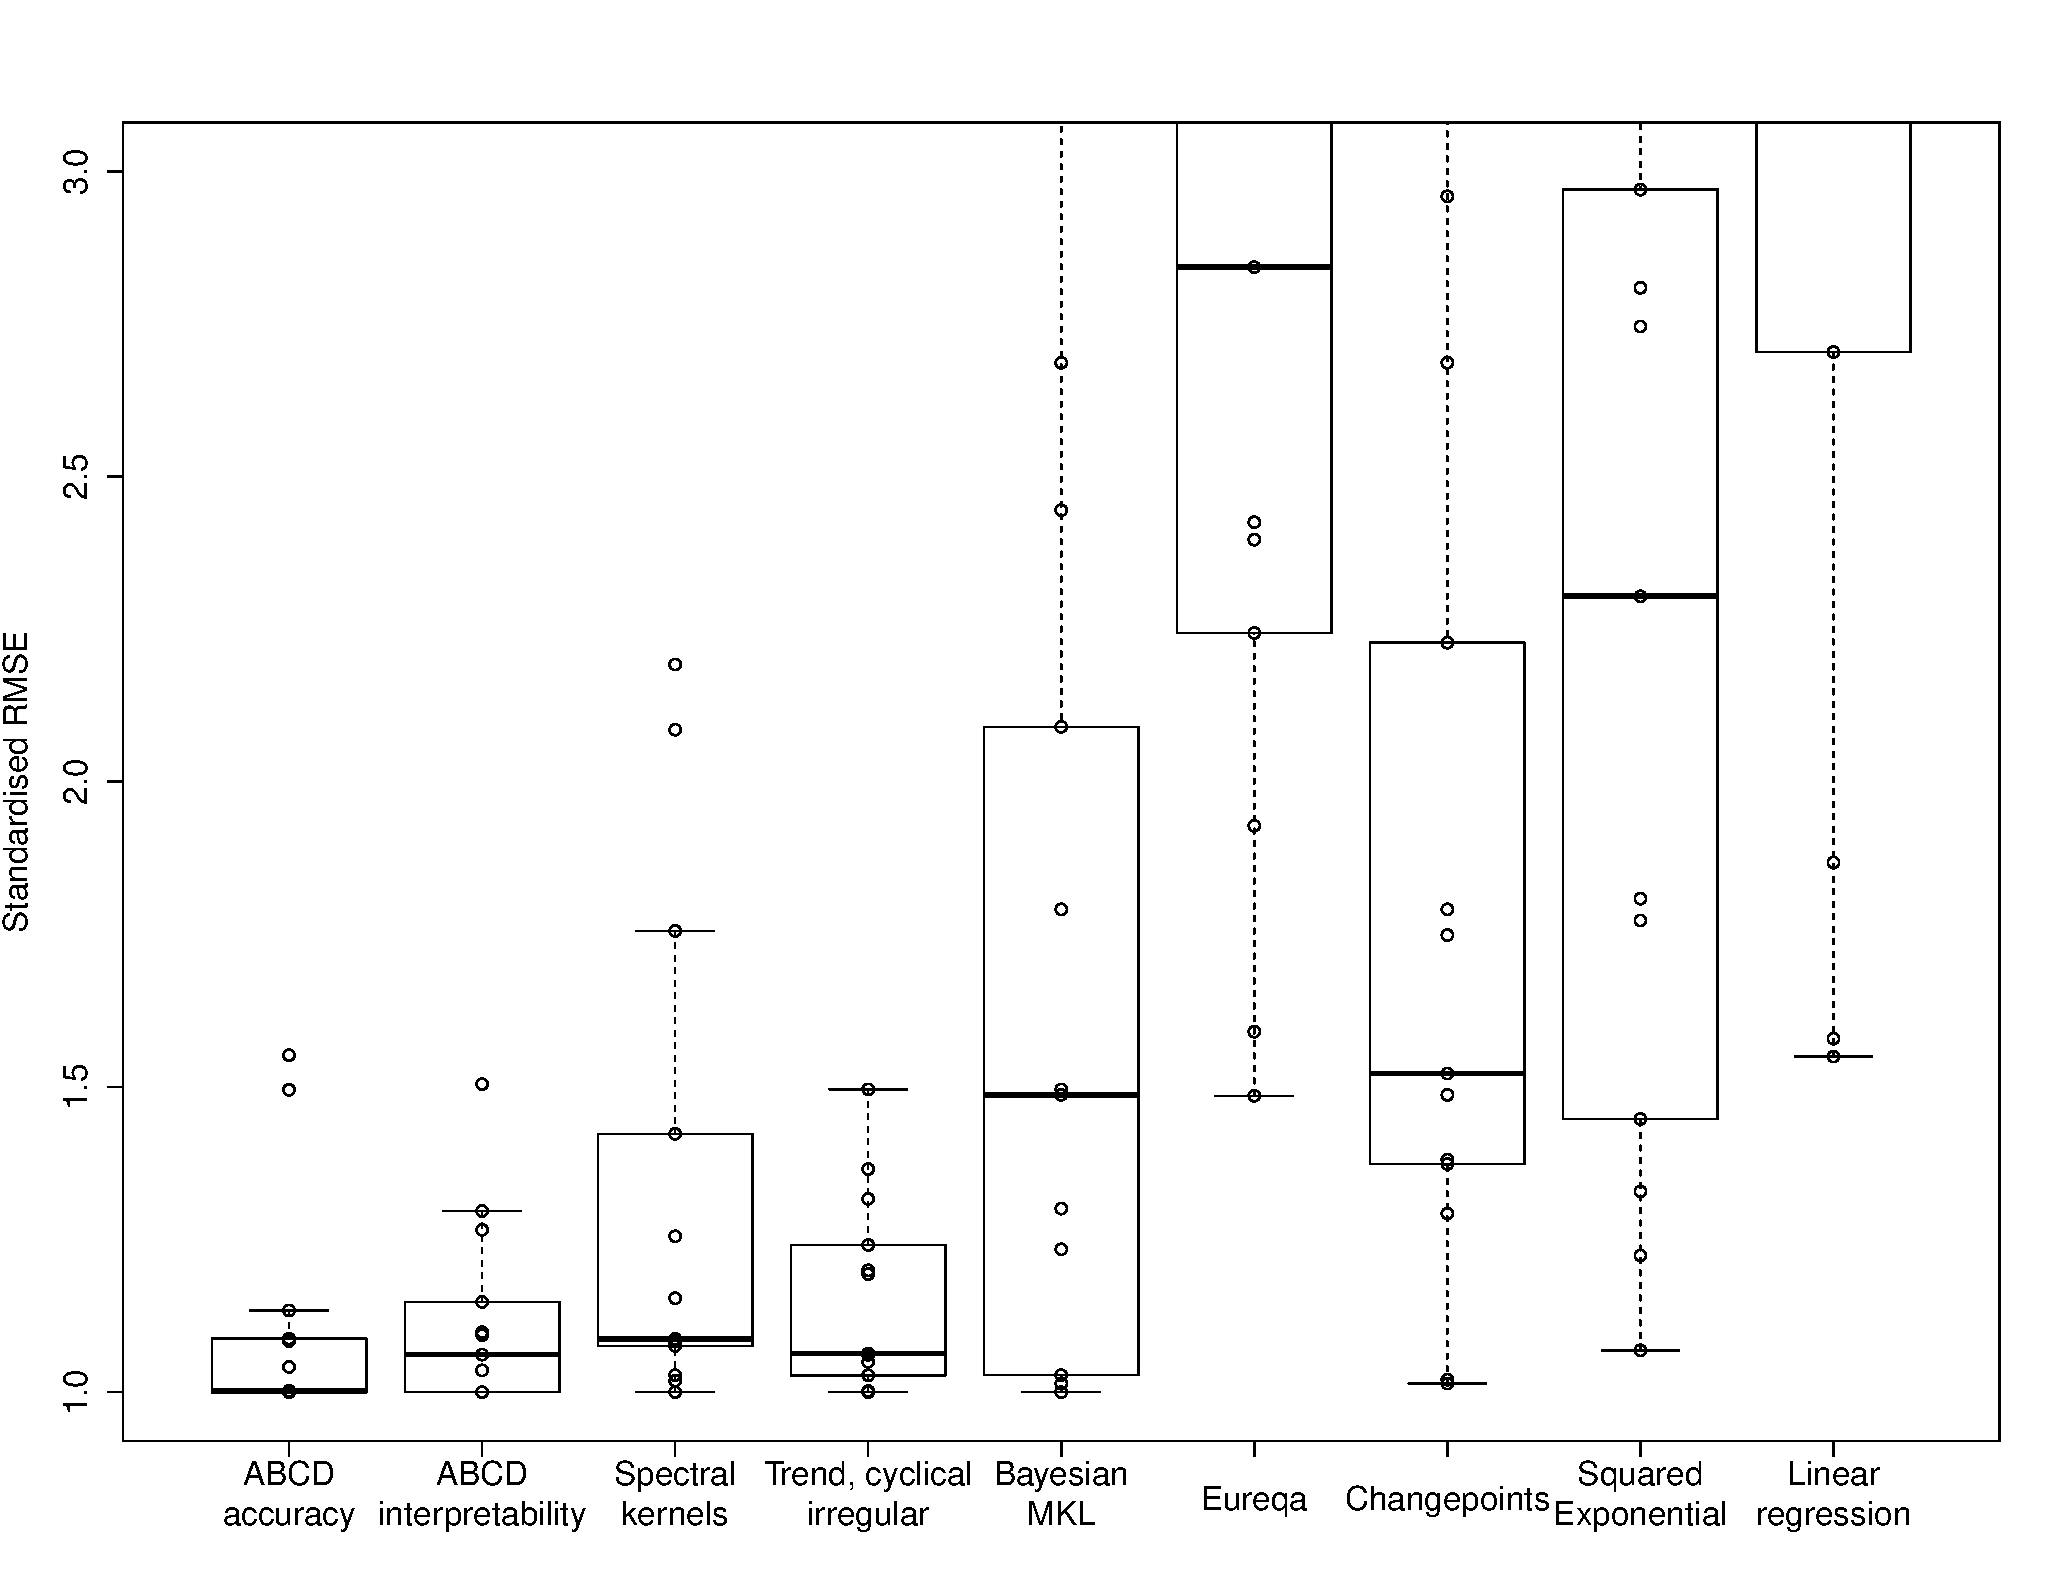
\includegraphics[width=\textwidth]{\grammarfiguresdir/comparison/box_interp}
\caption[Comparision of interpolation error of all methods on 13 time-series datasets.]
{Box plot of standardised \RMSE{} (best performance = 1) on 13 interpolation tasks.}
\label{fig:box_interp}
\end{figure*}

Changepoints performs slightly worse than \MKL{} despite being strictly more general than Changepoints.
The introduction of changepoints allows for more structured models, but it introduces parametric forms into the regression models (\ie the sigmoids expressing the changepoints).
This results in worse interpolations at the locations of the change points, suggesting that a more robust modeling language would require a more flexible class of changepoint shapes or improved inference (\eg fully Bayesian inference over the location and shape of the changepoint).

Eureqa is not suited to this task and performs poorly.
The models learned by Eureqa tend to capture only broad trends of the data since the fine details are not well explained by parametric forms.

\subsection{Tabels of standardised RMSEs}

See table~\ref{table:interp} for raw interpolation results and table~\ref{table:extrap} for raw extrapolation results. 
The rows follow the order of the datasets in the rest of the supplementary material.
The following abbreviations are used: \procedurename{}-accuracy (\procedurename{}-acc), \procedurename{}-interpretability ((\procedurename{}-int), Spectral kernels (SP), Trend-cyclical-irregular (TCI), Bayesian MKL (MKL), Eureqa (EL), Changepoints (CP), Squared exponential (SE) and Linear regression (Lin).

\begin{table*}[ht]
\center
\begin{tabular}{|c|c|c|c|c|c|c|c|c|}
\hline
\procedurename{}-acc & \procedurename{}-int & SP & TCI & MKL & EL & CP & SE & Lin \\
\hline
1.04 & 1.00 & 2.09 & 1.32 & 3.20 & 5.30 & 3.25 & 4.87 & 5.01\\
1.00 & 1.27 & 1.09 & 1.50 & 1.50 & 3.22 & 1.75 & 2.75 & 3.26\\
1.00 & 1.00 & 1.09 & 1.00 & 2.69 & 26.20 & 2.69 & 7.93 & 10.74\\
1.09 & 1.04 & 1.00 & 1.00 & 1.00 & 1.59 & 1.37 & 1.33 & 1.55\\
1.00 & 1.06 & 1.08 & 1.06 & 1.01 & 1.49 & 1.01 & 1.07 & 1.58\\
1.50 & 1.00 & 2.19 & 1.37 & 2.09 & 7.88 & 2.23 & 6.19 & 7.36\\
1.55 & 1.50 & 1.02 & 1.00 & 1.00 & 2.40 & 1.52 & 1.22 & 6.28\\
1.00 & 1.30 & 1.26 & 1.24 & 1.49 & 2.43 & 1.49 & 2.30 & 3.20\\
1.00 & 1.09 & 1.08 & 1.06 & 1.30 & 2.84 & 1.29 & 2.81 & 3.79\\
1.08 & 1.00 & 1.15 & 1.19 & 1.23 & 42.56 & 1.38 & 1.45 & 2.70\\
1.13 & 1.00 & 1.42 & 1.05 & 2.44 & 3.29 & 2.96 & 2.97 & 3.40\\
1.00 & 1.15 & 1.76 & 1.20 & 1.79 & 1.93 & 1.79 & 1.81 & 1.87\\
1.00 & 1.10 & 1.03 & 1.03 & 1.03 & 2.24 & 1.02 & 1.77 & 9.97\\
\hline
\end{tabular}
\caption[Interpolation error]{Interpolation standardised RMSEs}
\label{table:interp}
\end{table*}

\begin{table*}[ht]
\center
\begin{tabular}{|c|c|c|c|c|c|c|c|c|}
\hline
\procedurename{}-acc & \procedurename{}-int & SP & TCI & MKL & EL & CP & SE & Lin \\
\hline
1.14 & 2.10 & 1.00 & 1.44 & 4.73 & 3.24 & 4.80 & 32.21 & 4.94\\
1.00 & 1.26 & 1.21 & 1.03 & 1.00 & 2.64 & 1.03 & 1.61 & 1.07\\
1.40 & 1.00 & 1.32 & 1.29 & 1.74 & 2.54 & 1.74 & 1.85 & 3.19\\
1.07 & 1.18 & 3.00 & 3.00 & 3.00 & 1.31 & 1.00 & 3.03 & 1.02\\
1.00 & 1.00 & 1.03 & 1.00 & 1.35 & 1.28 & 1.35 & 2.72 & 1.51\\
1.00 & 2.03 & 3.38 & 2.14 & 4.09 & 6.26 & 4.17 & 4.13 & 4.93\\
2.98 & 1.00 & 11.04 & 1.80 & 1.80 & 493.30 & 3.54 & 22.63 & 28.76\\
3.10 & 1.88 & 1.00 & 2.31 & 3.13 & 1.41 & 3.13 & 8.46 & 4.31\\
1.00 & 2.05 & 1.61 & 1.52 & 2.90 & 2.73 & 3.14 & 2.85 & 2.64\\
1.00 & 1.45 & 1.43 & 1.80 & 1.61 & 1.97 & 2.25 & 1.08 & 3.52\\
2.16 & 2.03 & 3.57 & 2.23 & 1.71 & 2.23 & 1.66 & 1.89 & 1.00\\
1.06 & 1.00 & 1.54 & 1.56 & 1.85 & 1.93 & 1.84 & 1.66 & 1.96\\
3.03 & 4.00 & 3.63 & 3.12 & 3.16 & 1.00 & 5.83 & 5.35 & 4.25\\
\hline
\end{tabular}
\caption[Extrapolation error]{Extrapolation standardised RMSEs}
\label{table:extrap}
\end{table*}

\fi


\iffalse

\subsection{Comparison to Equation Learning}
\label{sec:eqn-learning-comp}

We now compare the descriptions generated by \procedurename{} to parametric functions produced by an equation learning system.
We show equations produced by Eureqa \citep{Eureqa} for the data sets shown above, using the default mean absolute error performance metric.

The learned function for the solar irradiance data is
\begin{align*}
\textrm{Irradiance($t$)} = 1361 + \alpha\sin(\beta + \gamma t)\sin(\delta + \epsilon t^2 - \zeta t)
\end{align*}
where $t$ is time and constants are replaced with symbols for brevity.
This equation captures the constant offset of the data, and models the long-term trend with a product of sinusoids, but fails to capture the solar cycle or the Maunder minimum.

The learned function for the airline passenger data is
\begin{align*}
\textrm{Passengers($t$)} = \alpha t + \beta\cos(\gamma - \delta t)\textrm{logistic}(\epsilon t - \zeta) - \eta
\end{align*}
which captures the approximately linear trend, and the periodic component with approximately linearly (logistic) increasing amplitude.
However, the annual cycle is heavily approximated by a sinusoid and the model does not capture heteroscedasticity.

\fi
